
\section{Reinforcement-learning model}
\label{sec:k-ase}

Depending on what information is provided to the learning agent, learning
methods can be grouped into three categories: supervised learning, unsupervised
learning and reinforcement learning.
Reinforcement learning is a compromise between supervised learning and
unsupervised learning. It learns to map situations to actions via online and
trial-and-error exploration. Instead of providing desired input/output pairs for
training, or no information other than the data, the environment provides a
feedback to the learning agent on how good the agent's outputs are after the
learning agent interacts with the environment.

\subsection{Architecture}

Our neural network architecture is based both on the box model proposed by
\cite{Michie68} and the ASE-ACE model proposed by \cite{Barto90}, as shown in
Figure~\ref{fig:kase}.

\begin{figure}[htb]
  \centering
  \psfrag{d}[bc]{\small$\Delta t$}
  \psfrag{ase}[bc]{\small$ASE$}
  \psfrag{ace}[bc]{\small$ACE$}
  \psfrag{t}[bc]{\small$\theta(t)$}
  \psfrag{tt}[bc]{\small$\theta$(t-$\Delta t$)}
  \psfrag{x}[bc]{\small$x(t)$}
  \psfrag{xx}[bc]{\small$\dot{x}(t)$}
  \psfrag{xxx}[bc]{\small$\ddot{x}(t)$}
  \psfrag{m}[bc][][1][90]{\small$Simulated$ $model$}
  \psfrag{k}[bc][][1][90]{\small$Kohonen$ $network$}
  \psfrag{+}[bc]{\small$+$}
  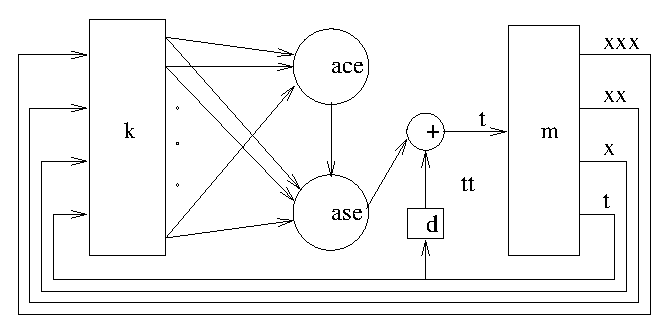
\includegraphics[width=0.9\columnwidth]{neural_network}
  \caption{Neural network architecture.}
  \label{fig:kase}
\end{figure}

The \emph{Simulated model} block reproduces the physics of the ball and plate
implementing the equations reported in Section~\ref{sec:sysmodel}.
According to its input, that is the updated plate angle, such a module
computes all the other system parameters which compose the system state $S$ as

$$S = [ \quad x \quad \dot{x} \quad \ddot{x} \quad \theta_x \quad ]^T.$$

The state $S$ is quantized through a \emph{Self Organizing Map} (SOM),
also known as \emph{Kohonen network}. 
The training parameters for such a network are reported in
Table~\ref{tab:kohonenparams}.
Note that a situation of $R_{min}$ equal to 1 implies that only the winning
neuron is updated.

\begin{table}
  \begin{center}
    \begin{tabular}{| l | c || r | }
      \hline
         $n$            & number of nodes                    & $700$ \\ \hline
         $n_r$          & number of rows                     & $35$  \\ \hline
         $n_c$          & number of columns                  & $20$  \\ \hline
         $\alpha_{max}$ & initial learning rate              & $0.4$ \\ \hline
         $\alpha_{min}$ & final learning rate                & $0.0$ \\ \hline
         $R_{max}$      & initial radius                     & $10$  \\ \hline
         $R_{min}$      & final radius                       & $1$   \\ \hline
         $T_{max}$      & max training duration (iterations) & $10^8$\\ \hline
    \end{tabular}
    \caption{Training parameters for the Kohonen network.}
    \label{tab:kohonenparams}
  \end{center}
\end{table}

The \emph{Associative Search Element} (ASE) associates a correct action in
response to a quantized input.
Moreover, the \emph{Adaptive Critic Element} (ACE) produces a secondary
reinforcement in order to let the ASE learn also when failures occur less
frequently.

The ASE's output consists of the plate angle variation, which is added to 
$\theta (t-\Delta t)$, to obtain the new plate angle.

The parameters of the \emph{Associative Search Element} (ASE) and
\emph{Adaptive Critic Element} (ACE) are reported respectively in
Table~\ref{tab:aseparams} and Table~\ref{tab:aceparams}. In order to
understand the meaning of such parameters, please refer to the handout
slides available at \cite{buttazzos_slides}.

\begin{table}
  \begin{center}
    \begin{tabular}{| l || r | }
      \hline
         $n$            & $700$ \\ \hline
         $\alpha$       & $10.0$ \\ \hline
         $\lambda$      & $0.75$ \\ \hline
    \end{tabular}
    \caption{ASE parameters.}
    \label{tab:aseparams}
  \end{center}
\end{table}

\begin{table}
  \begin{center}
    \begin{tabular}{| l || r | }
      \hline
         $n$            & $700$ \\ \hline
         $\lambda$      & $0.5$ \\ \hline
         $\beta$        & $0.4$ \\ \hline
         $\gamma$       & $1.0$ \\ \hline
    \end{tabular}
    \caption{ACE parameters.}
    \label{tab:aceparams}
  \end{center}
\end{table}

Initially, the failure condition was detected whenever the ball position hit
the plate borders.
Although this solution is simple and conceptually correct, unfortunately
it presents an unpleasant drawback, that is a slow and ineffective learning.
This effect is due to the fact that the simulations, in which the ball rolls 
from a border to another and back, are considered under control.
To avoid this kind of situation, the chosen approach consists in reducing
progressively the valid area during the simulation: at the beginning
such an area covers the whole plate; after a while, it shrinks proportionally
down to the lower bound. Each simulation not able to carry
the ball near the plate center in a limited time generates a failure.

